\chapter{相位扩散、模式耦合与预热化}
\label{ch:phase-dynamics}

\begin{learningobjectives}
完成本章后，读者应能：
\begin{enumerate}
  \item 区分全局相位扩散、有限波数去相位和非线性碰撞再分配；
  \item 由相对数涨落推导相干因子的高斯衰减；
  \item 用模式占据、反常关联和守恒量识别预热化时间窗；
  \item 说明为什么非线性 TWA 轨迹中的阻尼不能单独证明不可逆量子热化。
\end{enumerate}
\end{learningobjectives}

\section{三种容易混淆的“失相干”}

关闭线性耦合后，跨分量相干
\begin{equation}
  C_{LR}(t)=
  \frac{\int\dd x\,\qavg{\hat\Psi_L^\dagger(x,t)\hat\Psi_R(x,t)}}
  {\sqrt{\qavg{\hat N_L}\qavg{\hat N_R}}}
  \label{eq:intercomponent-coherence}
\end{equation}
通常下降，但至少有三种不同机制：
\begin{enumerate}
  \item \textbf{全局相位扩散}：不同相对粒子数分量具有不同化学势差；
  \item \textbf{线性模式去相位}：不同 $k$ 的稳定 Bogoliubov 模以不同频率旋转；
  \item \textbf{非线性模式耦合}：三波、四波过程改变模式占据并可能建立动理学松弛。
\end{enumerate}
它们可以在同一曲线上叠加，却对应不同可逆性、尺寸标度和理论近似。只拟合一个指数衰减常数不能识别机制。

跨分量算符 $\hat\Psi_L^\dagger\hat\Psi_R$ 已是两个不同正则模式的双线性乘积，其 Wigner 估计器直接是
$\ensavg{\psi_L^*\psi_R}$，没有同分量密度的半量子接触扣除。

\section{零模的相位扩散}

令相对数差为 $\delta N=(N_L-N_R)/2$，相对相位为
$\phi=\theta_R-\theta_L$。在小涨落集体坐标中，淬火前可写成
\begin{equation}
  H_{\rm rel}=\frac{E_C}{2}(\delta N)^2
  +\frac{E_J}{2}\phi^2,
  \label{eq:relative-collective-hamiltonian}
\end{equation}
其中 $E_J$ 来自式\eqref{eq:josephson-phase-energy}在极小值附近的展开。关闭 $J$ 后取 $E_J=0$，Hamilton 方程给出
\begin{equation}
  \delta N(t)=\delta N(0),
  \qquad
  \phi(t)=\phi(0)+\frac{E_Ct}{\hbar}\delta N(0).
  \label{eq:phase-diffusion-trajectory}
\end{equation}
若初态是高斯，便有
\begin{align}
  \Var[\phi(t)]={}&\Var[\phi(0)]
  +2\frac{E_Ct}{\hbar}\Cov[\phi(0),\delta N(0)]
  +\left(\frac{E_Ct}{\hbar}\right)^2\Var[\delta N(0)].
  \label{eq:phase-variance-growth}
\end{align}
当均值为零时，圆相干因子为
\begin{equation}
  \qavg{\ee^{\ii\phi(t)}}
  =\exp\!\left[-\frac12\Var[\phi(t)]\right].
  \label{eq:gaussian-phase-coherence}
\end{equation}
若初始交叉协方差可忽略，可定义尺度
\begin{equation}
  \tau_\phi=\frac{\hbar}{E_C\sqrt{\Var(\delta N)}}.
  \label{eq:phase-diffusion-time}
\end{equation}
它控制高斯包络，而不是普适的指数寿命。

相位扩散来自相对数的不确定度，但这里必须区分精确量子态与半经典相位包。精确的 $\delta N$ 本征态没有一个同时确定的共轭相对相位；其相位表象概率在圆上展开，不能把式\eqref{eq:phase-diffusion-trajectory}解释为“一个确定相位沿轨迹转动”。若初态是窄但非零宽度的数压缩半经典波包，且没有空间模式或其他噪声使化学势差变化，每个样本才近似作确定性转动，系综展宽由实际的 $\Var(\delta N)$ 决定。相干态抽样天然含相对数涨落；固定数差的精确态则需要周期相位表示或数守恒方法，普通 Cartesian 高斯近似只在远离圆周绕回且涨落近似连续的时间窗内适用。

有限量子转子的数谱离散，长时间可以出现回复。把 $\delta N$ 当连续变量的高斯 TWA 能准确描述早期展开，却通常丢失离散谱干涉造成的精确回复。这与第6章 Kerr 反例是同一种限制。

\section{空间相位场与线性去相位}

低能自旋通道可用相对相位 $\phi(x)$ 与相对密度 $s(x)$ 描述：
\begin{equation}
  H_s^{(2)}=\frac12\int\dd x\left[
  \chi_s^{-1}s(x)^2+\rho_s(\partial_x\phi)^2
  +M_J^2\phi(x)^2\right].
  \label{eq:spin-hydrodynamic-hamiltonian}
\end{equation}
$M_J$ 在耦合关闭后消失。每个稳定 Fourier 模都是独立谐振子；第15章的淬火协方差在这些模式中旋转。局域相干满足高斯恒等式
\begin{equation}
  \qavg{\ee^{\ii[\phi(x,t)-\phi(x',t)]}}
  =\exp\!\left[-\frac12
  \qavg{[\phi(x,t)-\phi(x',t)]^2}\right].
  \label{eq:gaussian-spatial-coherence}
\end{equation}
不同波数的非公度频率会使简单观测量趋于平滑平台，即使每个模式占据在严格二次理论中保持不变。这是相位混合或去相位，不是能量在模式间碰撞转移。

在近线性色散中，关联变化还会呈现有限传播速度形成的“光锥”结构。计算域必须大到使该前沿在分析窗口内不绕过周期边界。

\section{预热化平台}

若存在时间尺度分离
\begin{equation}
  \tau_{\rm dephase}\ll t\ll\tau_{\rm collision},
  \label{eq:prethermal-window}
\end{equation}
局域观测量可能已经近似平稳，而近似守恒的线性模式占据仍保留初态信息。这一中间状态称为预热化平台；孤立一维量子气体中已有相应实验观测\cite{Gring2012}。它常可由高斯协方差或广义统计系综描述，但“有效温度”可能依赖观测通道和波数范围。

识别预热化至少应同时展示：
\begin{enumerate}
  \item 一些实空间观测量已进入平台；
  \item 线性模式占据在该窗口内近似不变；
  \item 反常关联通过去相位下降或振荡平均；
  \item 更晚时非线性占据再分配尚未显著；
  \item 平台随系统尺寸和截止的变化受控。
\end{enumerate}

\section{非线性模式耦合}

把完整哈密顿量在凝聚背景附近展开，除了 $H^{(2)}$ 外还有
\begin{equation}
  H=H^{(0)}+H^{(2)}+H^{(3)}+H^{(4)}+\cdots.
\end{equation}
$H^{(3)}$ 允许满足能量--动量条件的一模衰变为两模及其逆过程，通常与 Beliaev 和 Landau 过程相关；$H^{(4)}$ 产生四波散射与频率重整化。是否存在共振取决于实际色散、维数、陷阱和 SOC，自旋“Cherenkov 发射”不是所有双分量模型的普适标签。

非线性 GPE/TWA 轨迹确实包含这些经典场模式耦合顶角，无需手工附加碰撞项。但由此观察到模式占据变化，只能说明所模拟的截断经典场发生了再分配。要把速率解释成量子 Beliaev--Landau 碰撞，还需在弱耦合重叠区与量子动理学或微扰计算比较，并检查每个参与模式的占据与截止依赖。

\section{“不可逆”需要操作定义}

闭合 TWA 轨迹的 Hamilton 流是微观可逆的。若保存终态并用负时间步长精确反演，理想数值程序应回到初态；系综平均阻尼来自相空间剪切、混合和信息粗粒化。真正的实验不可逆性可以由不可控自由度、开放系统或热力学极限中的极长回归时间产生，但不能由一条平滑衰减曲线单独证明。

可以设计三类区分实验：
\begin{enumerate}
  \item \textbf{回波}：在 $t_e$ 反转可控 Hamilton 参数，检查相干是否恢复；
  \item \textbf{占据账本}：区分固定占据的去相位与随时间改变的碰撞再分配；
  \item \textbf{分布检验}：比较晚时模式分布与 Bose--Einstein、Rayleigh--Jeans 及广义系综，并做截止稳定性。
\end{enumerate}
TWA 的晚时经典场常趋向截止相关的 Rayleigh--Jeans 型分布，因此仅凭“拟合出温度”不能声称量子热化。

\section{实际相位扩散基准}

配套程序对式\eqref{eq:phase-diffusion-trajectory}抽样 $2\times10^5$ 条高斯轨迹，并与式\eqref{eq:phase-variance-growth}和\eqref{eq:gaussian-phase-coherence}比较，结果见\cref{fig:phase-diffusion-benchmark}。
\begin{figure}[htbp]
  \centering
  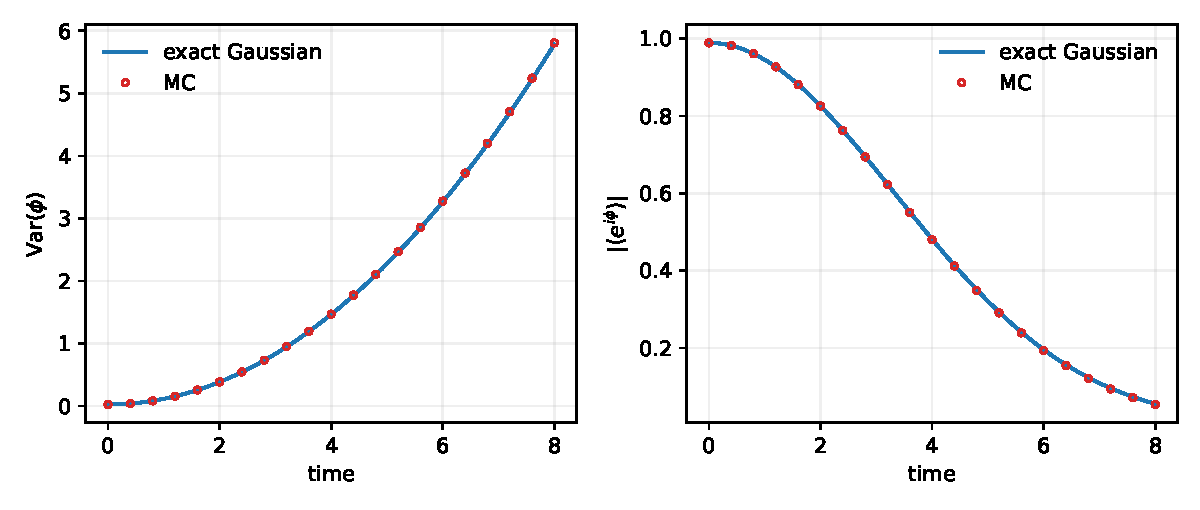
\includegraphics[width=0.78\textwidth]{figures/ch16/phase_diffusion.pdf}
  \caption[相对相位扩散的高斯 Monte Carlo 基准]{相对相位扩散的解析式与 Monte Carlo 对照。参数为 $E_C=0.1$、$\sigma_N=3$、$\sigma_\phi=0.15$，点和 $\pm1$ 标准误来自 $200000$ 条高斯轨迹；相位方差与相干包络的最大偏差分别为 $1.36$、$1.51$ 个标准误以内。该图只检验可逆零模剪切，不含空间传播、碰撞或耗散。}
  \label{fig:phase-diffusion-benchmark}
\end{figure}
图中相干衰减完全来自相对数导致的可逆相空间剪切，没有加入碰撞或耗散。指标保存在
\path{data/ch16/phase_diffusion_metrics.json}。

\section{端到端空间场淬火基准}

前一个基准只检验零模解析公式。为把第10--15章的环节真正接起来，配套程序
\path{code/ch14_17_capstone/two_component_field_quench.py}
执行一次受限但完整的双分量空间场计算：在 $\hbar=m=1$ 的单位中取周期长度 $L=32$、$64$ 个格点、凝聚背景总密度参数 $n=12$、$g=0.05$、$g_{12}=0.035$、$T=0.30$，先在 $J_i=0.15$ 的稳定密度/自旋 BdG 基中抽样有限温 Wigner 噪声，再突然关闭均匀 Rabi 耦合到 $J_f=0$，最后用含 Weyl 基线的双分量 Strang 分步法传播。这里 $n$ 是展开点的凝聚背景密度，$nL=384$ 不是抽样后的正规排序总粒子数；后者的系综均值为 $406.83$，还包含该有限 BdG 基中的量子与热耗尽。

密度 $k=0$ 是 Goldstone 坐标，不能代入普通热 BdG 振子公式。这里把它定义成承载宏观位移的凝聚相干零模，并抽样其真空 Wigner 噪声，即 $\ensavg{|b_{d,0}|^2}=1/2$、$\ensavg{b_{d,0}^2}=0$，但不赋予热 BdG 占据；有隙自旋零模则仍按有限温 BdG 协方差抽样。因此密度/自旋两个通道的全部 $2N_x$ 个模式都各自带有相应的 Wigner 半量子，与排序基线所计数的 $2N_x$ 个正则原子模式逐一对应。这个方案并不固定总粒子数：宏观零模的真空噪声会产生真实的样本间总数涨落，不能再称作数守恒抽样；本次初态正规排序总数在 $256$ 个样本间的标准差为 $26.67$，即均值的 $6.56\%$（其中也含其余密度模的量子与热涨落）。程序逐模检查 $b_k$ 的正常矩与 $b_kb_{-k}$ 反常矩，并在变换到原子密度/自旋通道后再次检查目标协方差；本次最大标准化残差分别为 $3.65$ 和 $3.66$，均低于预先写入指标文件的 $5$ 标准误门槛。Fourier 完备性、通道幺正性和 BdG 辛归一化的最大代数残差为 $3.7\times10^{-15}$。

观测量不是逐轨迹归一化后再平均，而是式\eqref{eq:intercomponent-coherence}对应的比值--系综估计器
\begin{equation}
  C_{LR}^{\rm est}(t)=
  \frac{\ensavg{\int\dd x\,\psi_L^*(x,t)\psi_R(x,t)}}
  {\sqrt{\ensavg{N_{L,W}}\ensavg{N_{R,W}}}},
  \qquad
  N_{\sigma,W}=\int\dd x\left(|\psi_\sigma|^2-\frac12\delta_{\mathcal C}\right).
  \label{eq:capstone-coherence-estimator}
\end{equation}
同时计算最低非零波矢 $k_1=2\pi/L$ 的正规排序自旋结构因子。这里两个
分量共有 $2N_x$ 个正则格点模式，故原始对称范数与数算符 Weyl 符号的关系是
\begin{equation}
  \mathcal N_{\mathrm{sym}}^{(s)}=\Delta x\sum_j
  (|\psi_{L,j}^{(s)}|^2+|\psi_{R,j}^{(s)}|^2),
  \qquad
  N_W^{(s)}=\mathcal N_{\mathrm{sym}}^{(s)}-N_x.
  \label{eq:capstone-number-symbol}
\end{equation}
关闭耦合后，程序还直接计算与同一有限格点基一致的离散 Weyl 哈密顿量
\begin{align}
  H_W={}&\sum_k\epsilon_k
  \left(|a_{L,k}|^2+|a_{R,k}|^2-1\right) \notag\\
  &+\frac{g\Delta x}{2}\sum_j\left[
  n_{L,j}^2+n_{R,j}^2-2\delta_{\mathcal C}(n_{L,j}+n_{R,j})
  +\delta_{\mathcal C}^2\right] \notag\\
  &+g_{12}\Delta x\sum_j
  \left(n_{L,j}-\frac{\delta_{\mathcal C}}2\right)
  \left(n_{R,j}-\frac{\delta_{\mathcal C}}2\right),
  \qquad n_{\sigma,j}=|\psi_{\sigma,j}|^2,
  \label{eq:capstone-discrete-weyl-hamiltonian}
\end{align}
其中 $a_{\sigma,k}$ 采用与实空间格点正交归一的 Fourier 约定，且
$\delta_{\mathcal C}=1/\Delta x$。动能中的 $-1$ 正是两个分量各自的半量子；相互作用项的线性项与常数项也不能遗漏，否则“能量守恒”检查的对象就不是实际传播的 Weyl 哈密顿量。
对同一完整正交格点基，结构因子的乘积估计器要扣除 $N_x/2$：
\begin{equation}
  S_s(k_1)=\frac{\ensavg{|S_{k_1,W}|^2}-N_x/2}{\ensavg{N_W}},
  \qquad
  S_{k,W}=\Delta x\sum_j\ee^{-\ii kx_j}
  (|\psi_{L,j}|^2-|\psi_{R,j}|^2).
  \label{eq:capstone-spin-structure-estimator}
\end{equation}

完整结果汇总于\cref{fig:two-component-field-capstone}。
\begin{figure}[htbp]
  \centering
  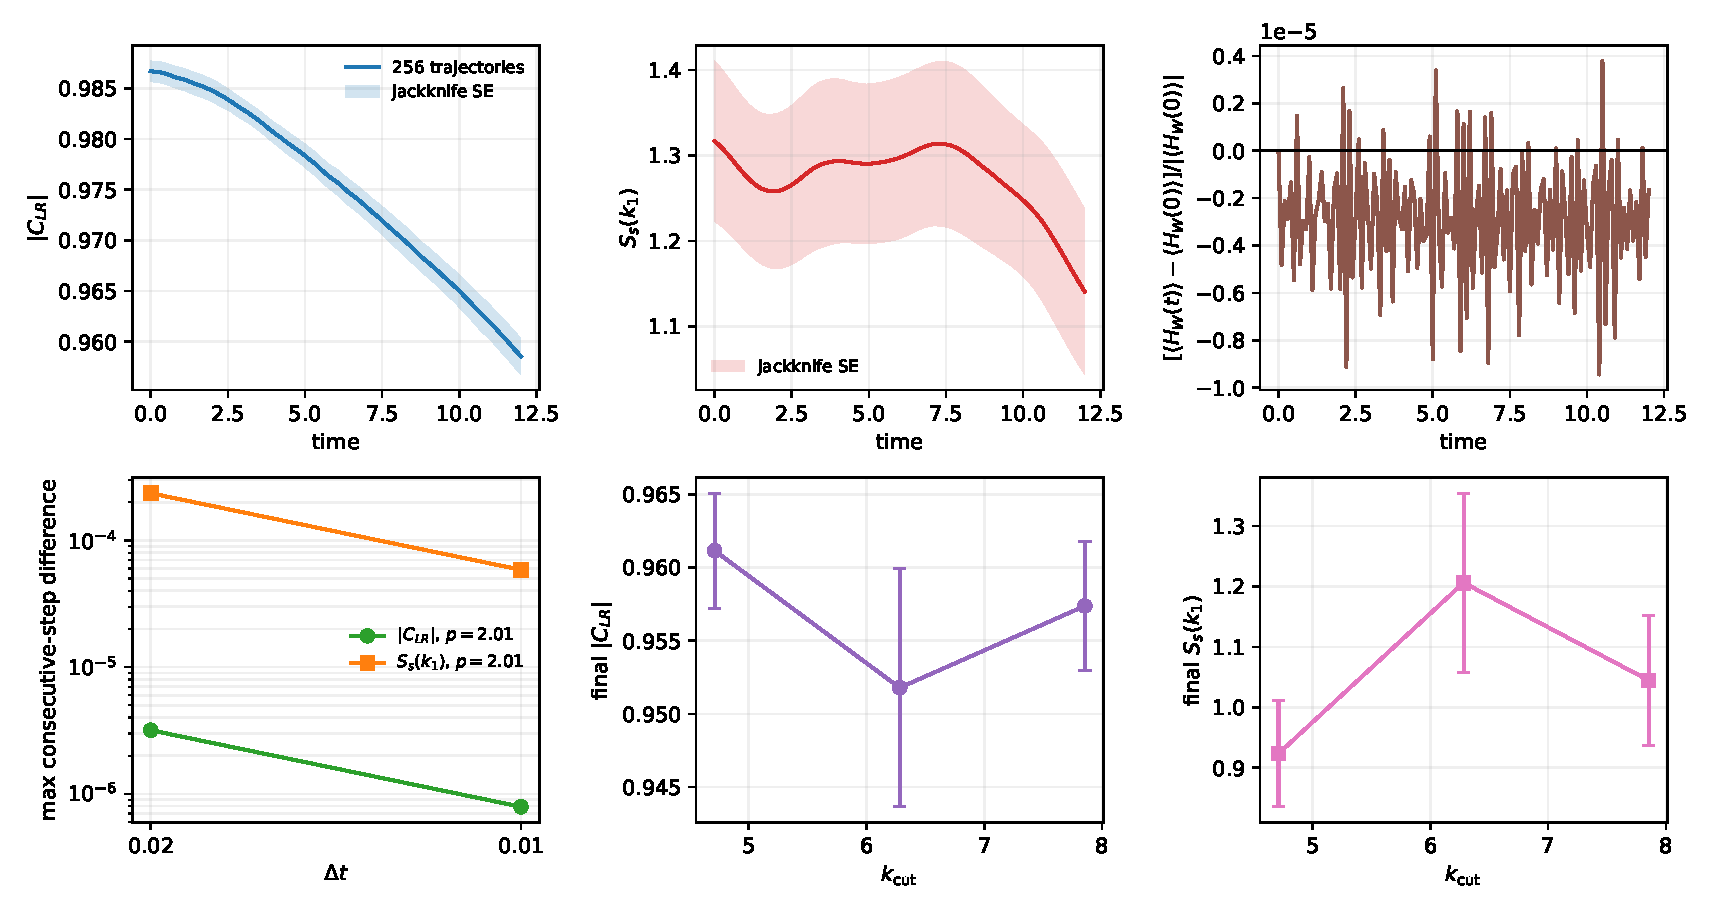
\includegraphics[width=0.96\textwidth]{figures/ch14_17_capstone/two_component_field_quench.pdf}
  \caption[双分量空间场淬火的端到端基准]{均匀 Rabi 双分量场从 $J_i=0.15$ 淬火到 $J_f=0$ 的端到端基准。生产曲线使用 $L=32$、$N_x=64$、$256$ 条轨迹，阴影为 $\pm1$ 删除分块 jackknife 标准误；其余面板显示离散 Weyl 能量漂移、$\Delta t=0.02,0.01,0.005$ 的二阶标度，以及 $N_x=48,64,80$ 截止压力测试（每档64条独立轨迹，误差棒为 $\pm1$ 标准误）。抽样的128个通道模式与排序基线一致，20项机器门禁全部通过。该结果只支持所测试有限时间和截止窗内的空间去相位与估计器闭环，不是 Raman SOC、预热化平台、热化或网格极限的证据。}
  \label{fig:two-component-field-capstone}
\end{figure}
在 $256$ 条轨迹中，$|C_{LR}|$ 从 $0.9867$ 降到 $0.9586$。相干曲线的删除分块 jackknife 标准误最大为 $1.79\times10^{-3}$，所以这一下降在本样本中清楚可分辨。最低非零波矢的 $S_s(k_1)$ 从 $1.317$ 变到 $1.141$，但它的全曲线 jackknife 标准误最大为 $0.098$；图中的误差带表明，当前轨迹数还不足以把每个细小振荡都解释成确定的空间模式信号。因而 $S_s(k_1)$ 在这里首先是排序修正与不确定度传播的实际场估计器验收，而不是独立的预热化证据。

用相同初态噪声比较 $\Delta t=0.02,0.01,0.005$，相干与 $S_s(k_1)$ 的连续差分都给出 Strang 观测阶 $2.01$；最细两档的最大曲线差分别为 $7.91\times10^{-7}$ 和 $5.86\times10^{-5}$，远小于相应 Monte Carlo 误差。把轨迹数从 $256$ 降至 $128$ 时，两条曲线的最大变化分别相当于 $1.29$ 和 $1.56$ 个 $256$ 轨迹最大 jackknife 标准误。总物理粒子数最大相对漂移为 $1.01\times10^{-13}$。式\eqref{eq:capstone-discrete-weyl-hamiltonian}的系综平均相对漂移不超过 $9.44\times10^{-6}$，单轨迹漂移的均方根不超过 $8.42\times10^{-5}$；共同噪声下每次把步长减半，系综能量漂移分别缩小到前一档的 $0.246$ 和 $0.249$，与二阶分步误差一致。

程序还在同一 $L$ 和已验收的 $\Delta t=0.005$ 下，对 $N_x=48,64,80$ 三个模式截止各自独立重新抽样 $64$ 条轨迹。终态相干分别为 $0.9611\pm0.0039$、$0.9518\pm0.0081$ 和 $0.9574\pm0.0044$，最大两两差异为 $1.04$ 个合并标准误；终态 $S_s(k_1)$ 分别为 $0.923\pm0.088$、$1.206\pm0.148$ 和 $1.045\pm0.108$，最大两两差异为 $1.64$ 个合并标准误。三档的系综平均 Weyl 能量最大相对漂移均不超过 $1.37\times10^{-5}$。由于三档数据不是嵌套样本、统计精度有限且没有显示单调趋势，这只是给定有限截止窗内未检出显著差异的压力测试，不能称作网格极限收敛。完整曲线、参数、随机种子、逐模矩、零模处理清单、结构化阈值与验收结果和截止数据保存在
\path{data/ch14_17_capstone/two_component_field_quench_metrics.json}。

这个结果只支持“在已测试的有限截止窗和有限时间内观察到空间场去相位”的结论。它没有做高精度截止外推和系统尺寸扫描，也没有展示随时间演化的模式占据在平台内保持、随后碰撞再分配，因此\emph{不是}预热化平台、更不是量子热化的证据；它也使用均匀 Rabi 模型而非 Raman SOC。初态的逐模正常矩与反常矩在这里只是抽样门禁，不能替代上述动力学证据。要把结论升级为预热化，至少还要输出这些矩的时间序列，识别式\eqref{eq:prethermal-window}的时间尺度分离，并扩大截止与尺寸扫描。

\section{从轨迹提取相对相位}

低密度点的局域相位噪声会发散，直接平均
$\arg\psi_R(x)-\arg\psi_L(x)$ 不稳健。全局相位可由复重叠
\begin{equation}
  A_{LR}^{(s)}(t)=\int\dd x\,
  \psi_L^{(s)*}(x,t)\psi_R^{(s)}(x,t),
  \qquad
  \phi_s=\arg A_{LR}^{(s)}
  \label{eq:trajectory-relative-phase}
\end{equation}
定义，并用圆统计量
\begin{equation}
  R_\phi=\left|\frac1{N_s}\sum_s\ee^{\ii\phi_s}\right|
  \label{eq:circular-resultant}
\end{equation}
衡量相位锁定。均匀分布在有限样本下也给出正的 $R_\phi$，应通过随机均匀相位空模型或已知的圆统计分布校准，而不是把任何非零值解释为残余相干。

\begin{chaptercheck}
当相干因子下降时，同时画出：相对相位圆分布、零模相对数、各 $k$ 正常占据、反常关联、总能量和反向传播误差。只有这些量的联合变化才能区分相位扩散、线性去相位、非线性再分配和数值伪阻尼。
\end{chaptercheck}

\section*{本章小结}

全局相位扩散由相对数不确定度造成，高斯相干包络可由协方差精确预测；空间模式的线性去相位可以产生预热化平台，却不改变二次理论中的模式占据。非线性场方程包含模式耦合，但 TWA 晚时阻尼仍可能是可逆混合或截止相关经典化。碰撞热化与不可逆性需要回波、占据再分配、分布和独立量子方法共同支持。

\begin{exercises}
  \item 从式\eqref{eq:phase-diffusion-trajectory}推导含非零初始交叉协方差的式\eqref{eq:phase-variance-growth}。
  \item 对精确固定相对数态解释为什么不能同时指定一条确定初始相位轨迹；再说明窄数压缩波包何时可近似使用高斯相位扩散公式。
  \item 在二次模式理论中证明正常模式占据不变而反常矩发生相位旋转。
  \item 设计一个回波协议，分别对纯去相位与弱碰撞情形给出预期结果。
  \item 提出至少三项证据，区分 Bose--Einstein 热分布与截止相关 Rayleigh--Jeans 分布。
  \item 扩展端到端空间场程序，输出淬火后密度/自旋 BdG 模的正常占据和反常矩，并据此检验是否存在式\eqref{eq:prethermal-window}，而不是仅凭 $C_{LR}(t)$ 命名预热化。
\end{exercises}
